\chapter{GUI}
\begin{center}
   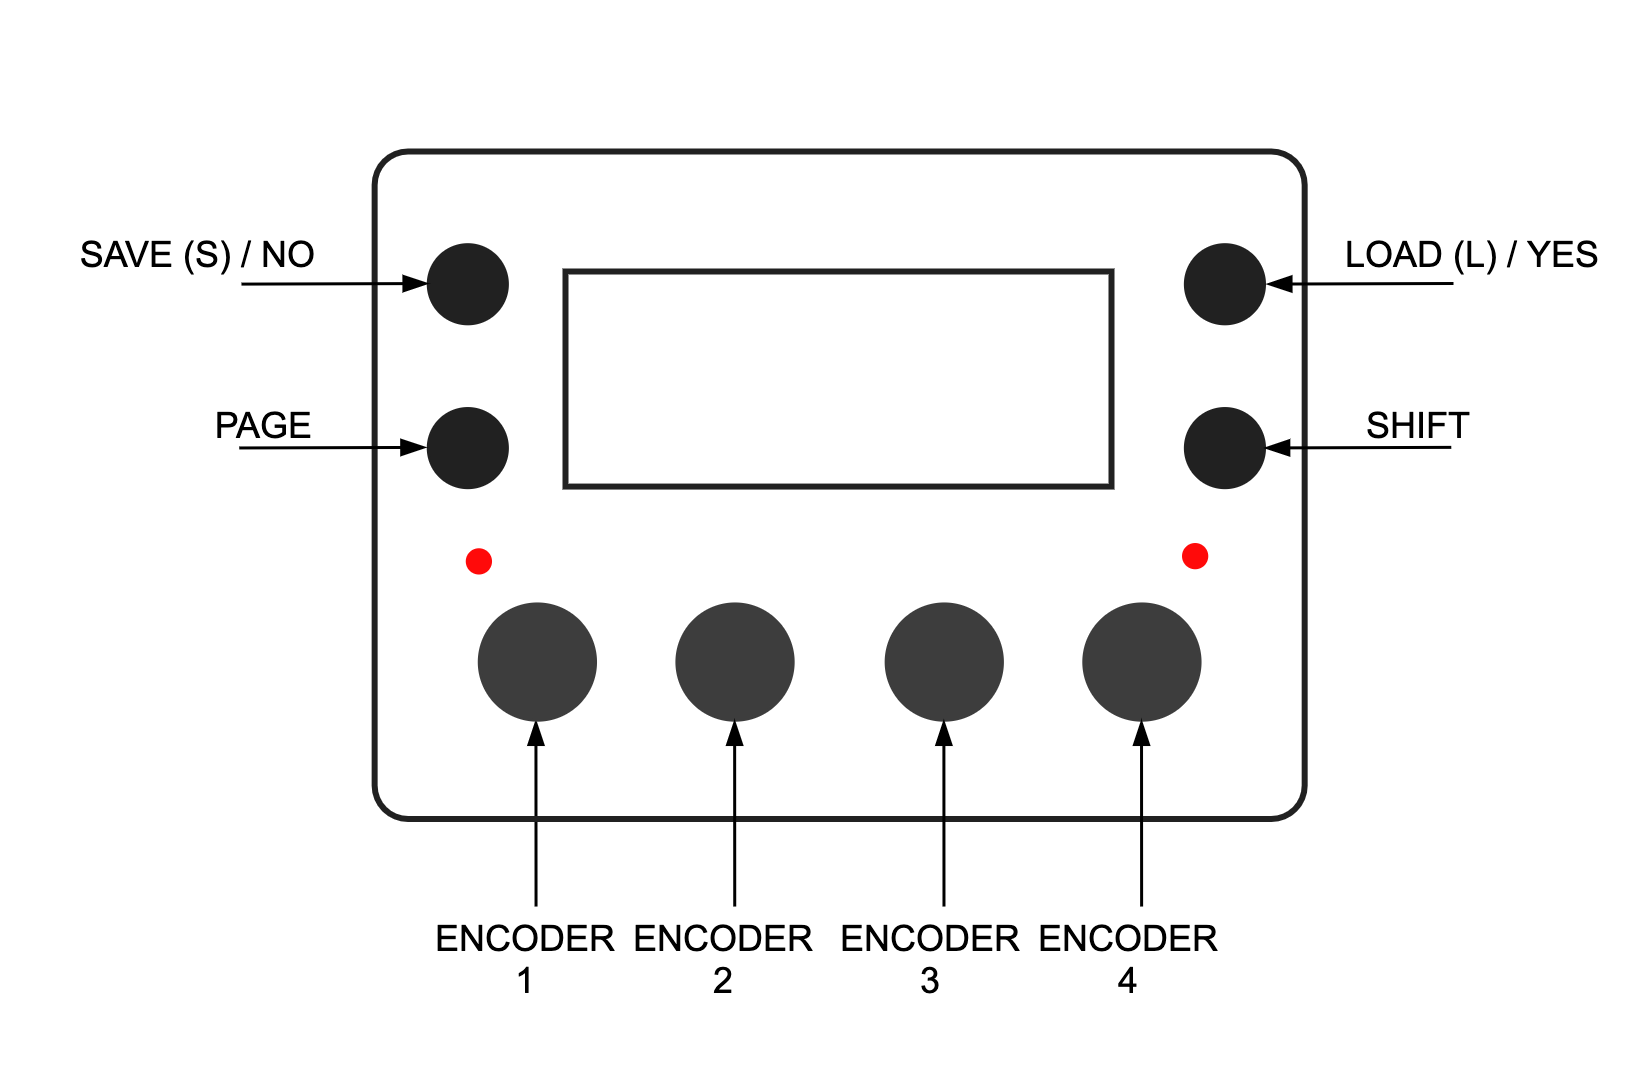
\includegraphics[width=18cm]{megacommand_gui.png}
\end{center}
\section{Function Buttons:}
From the Grid Page the MC's function buttons perform the following actions:
\begin{itemize}
\item{\textbf{<Save | No>}: Enters the Save Page.}
\item{\textbf{<Load | Yes>}: Enters the Load page.}
\item{\textbf{<Page>}: Enters the PageSelect page.}
\item{\textbf{<Shift | Menu>}: Opens the slot Menu. }
\end{itemize}
Combined Button Presses:
\begin{itemize}
\item{\textbf{<Save | No> + <Load | Yes>}: Opens the MCL Configuration menu. }
\end{itemize}

\section{Encoder Buttons}
Encoder buttons are used to increase the speed of parameter rotation.
Holding down an encoder button whilst rotating the encoder will increase the update speed by 4x.

\newpage
\section{Machinedrum GUI: Enhanced Mode}
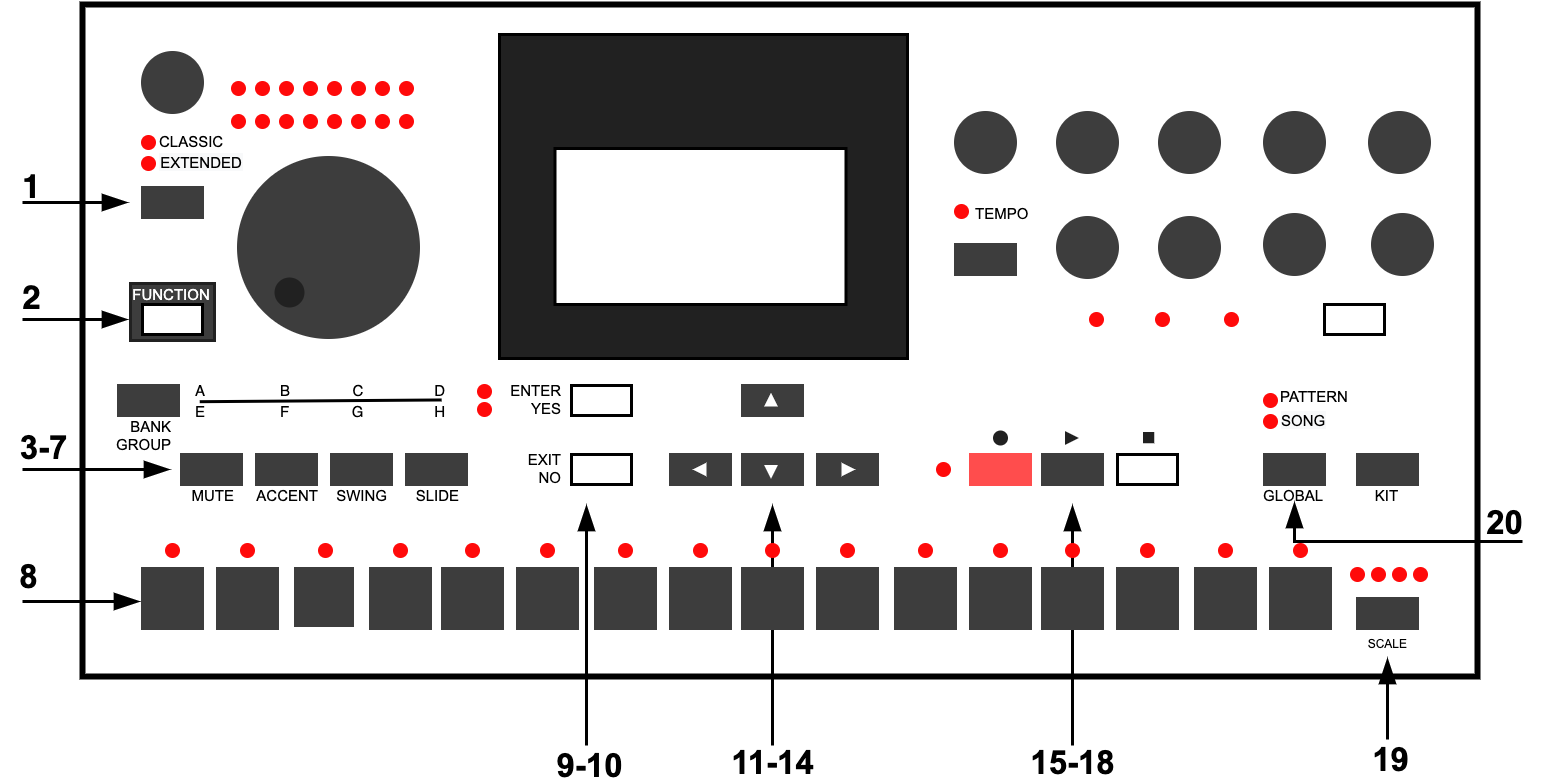
\includegraphics[width=18cm]{machinedrum_gui.png}

The MDX firmware introduces a third editing mode beyond Classic and Extended termed \textbf{Enhanced Mode}.\\
\\
Enhanced mode is activated automatically when the MD is connected to the MegaCommand.\\
\\
When in Enhanced mode, both Classic and Extended LEDs will be lit. The three modes can be toggled whilst the sequencer is stopped, by pressing the MD's \textbf{[Classic/Extended]} key.\\
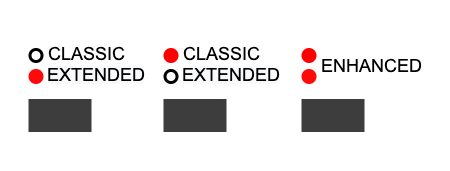
\includegraphics[width=10cm]{enhanced_mode.png}\\
Enhanced mode disables editing access to the MD's internal sequencer and enables the Machinedrum's GUI to be fully integrated with MCL.
\\\\
\textit{When using MCL with your MD, it is recommended that you first switch to Classic or Extended and load a blank pattern, then switch back to Enhanced mode. The MD's internal sequencer is never fully disabled, and the MCL sequencer will play alongside it.\\\\
The KitName + Pattern fields shown on the MD display are re-purposed to illustrate the position and name of MCL's last loaded row.
}
\newpage
\section{MD + MCL command summary}

\textbf{General:}
   \begin{itemize}
      \item \textbf{[Classic/Extended] } toggle between Classic, Extended and Enhanced Modes.\\(When in Enhanced mode, the sequencer must be stopped to switch modes.)
      \item \textbf{[Function] + [Bank Group]} toggle Bank Group selection.
      \item \textbf{[Rec]} Enter Step edit mode.
      \item \textbf{[Global]} Open the current Page's shift menu.
      \item \textbf{[Global] + [Up/Down/Left/Right]} Navigate the shift menu.
      \item \textbf{[Bank Group]} Hold to Open the Page Select menu.
      \item \textbf{[Bank Group] + [Trig]} MCL Page Select.
      \item \textbf{[Bank Group] + [Global]} MCL Config Menu. 
      \item \textbf{[Bank Group] + [Exit/No]} Return to Grid page
      \item \textbf{[Function] + [Encoder]} Simultaneously modify parameters across all tracks. 
       \item \textbf{[Function] + [Classic/Extended]} Simultaneously reset parameters to last load value across all tracks.
 \end{itemize}
 
\textbf{Loading:}
   \begin{itemize}
      \item \textbf{[Bank] + [Trig]} loads slots from the selected row according to Group selection.
      \item \textbf{[Bank] + [Multiple Trigs]} creates a chain of slots from selected rows according to Group selection.
   \end{itemize}

\textbf{Grid Page:}
    \begin{itemize}
      \item \textbf{[Up/Down/Left/Right]} position grid cursor. 
      \item \textbf{[Function] + [Up/Down/Left/Right]} grid cursor position fast travel.
      \item \textbf{[Scale]} Toggle active grid X or Y. 
      \item \textbf{[Function] + [Clear/Copy/Paste]} Clear/Copy/Paste  the MD tracks, EXT MIDI tracks and MD Master FX currently loaded in the sequencer.
      \item \textbf{[Function] + [Scale]} open "Scale Setup" menu adjust current track's length and speed settings.
      \item Hold \textbf{[Exit/No]} key to open Slot Menu.
      \begin{itemize}
                \item \textbf{[Bank A,B,C]} keys can be used to select load mode: MAN, AUT, QUE.
                \item \textbf{[Up/Down/Left/Right]} to select multiple slots in the grid.
                \item \textbf{[Clear/Copy/Paste]} to clear/copy/paste selected slot(s).
                \item \textbf{[Enter/Yes]} load selected slots. Slots are loaded according to the current load MODE setting. If more than one row is selected, the MODE is automatically set to QUE, and the loaded slots are added to each column's playback queue.                
      \end{itemize}

\textbf{[Enter/Yes]} opens \textbf{Load Page:}
    \begin{itemize}
    \item Hold \textbf{[Enter/Yes]} to open slot Group Select. Release \textbf{[Enter/Yes]} to load by group. Group selection is editable via \textbf{[Trig]} keys 1-5.
    \item \textbf{[Trig]} keys are used to select and load sequencer tracks from slots of the current row.
    \item \textbf{[Bank]} keys can be used to quickly select the load mode: MAN, AUT, QUE.
    \end{itemize}
    
\textbf{[Function] + [Enter/Yes]} opens \textbf{Save Page:}
    \begin{itemize}
    \item Hold \textbf{[Enter/Yes]} to open slot Group Select. Release \textbf{[Enter/Yes]} to save by group.  Group selection editable via \textbf{[Trig]} keys 1-5.
    \item \textbf{[Trig]} keys are used to select and save individual sequencer tracks to slots of the current row. If none are selected entire row (pattern) will be saved.
    \end{itemize}
\end{itemize}

\textbf{Mixer Page:}
      \begin{itemize}
       \item \textbf{[Scale]} Switch Grid X Y tracks.
       \item \textbf{[Trig]} Select track
       \item \textbf{[Trigs] + [Encoder]} Simultaneously modify parameters across selected tracks. 
       \item \textbf{[Trigs] + [Classic/Extended]} Simultaneously reset parameters to last load value across selected tracks.
       \item \textbf{[Trig]} + \textbf{[Enter/Yes]} Mute selected track(s).
      \item \textbf{[Trig]} + \textbf{[Exit/No]} Solo selected track(s).
      \item \textbf{[Function]} + \textbf{[Enter/Yes]} Flip active mutes.
      \item \textbf{[Up/Down/Left/Right]} Preview and edit mute sets.
      \item \textbf{[Up/Down/Left/Right] + [Enter/Yes]} Load selected mute set.
      \item \textbf{<Encoders1-4>} Performance Controllers (A,B,C,D) scene morphs.
      \item \textbf{[Up/Down/Left/Right] + [Exit/No] + <Encoders1-4>} Set performance controller lock to mute set.
      \item \textbf{[Function] + <Encoders1-4>} Hard pan performance controller left or right.
      \item \textbf{[Trig]} + \textbf{[Global]} Sequencer mute record for selected tracks.
      \item \textbf{[Trig]} + \textbf{[Kit]} Clear sequencer mute record for selected tracks
      \item \textbf{[Global]} + \textbf{[Kit]} Clear all active sequencer mute recordings.
      \item \textbf{[Exit/No] + [Left]} Toggle DELAY pages.
      \item \textbf{[Exit/No] + [Down]} Toggle REVERB pages.
       \end{itemize}
\newpage
\textbf{Performance Page:}
\begin{itemize}
      \item \textbf{[Global]} Open Performance menu.
      \item \textbf{[Global] + [Trig1-4]} Select active controller 1-4.
      \item \textbf{[Left] + [Trig1-8]} Set active controller LEFT scene 1-8.
      \item \textbf{[Right] + [Trig1-8]} Set active controller RIGHT scene 1-8.
      \item \textbf{[Trig] + [MD Encoder] Or Ext Midi Controller} Assign lock to scene.
      \item \textbf{[Trig] + [Clear/Copy/Paste]}Clear, Copy, Paste scenes (repeat to UNDO).
      \item \textbf{[Trig] + [Enter/Yes]} Scene preview.
      \item \textbf{[Trig] + [Up/Down]} View and edit 16 active scene locks.
      \end{itemize}
   \textbf{Route Page:} 
\begin{itemize}

     \item \textbf{[Trigs] }Toggle between Main output (--) and selected Route output on chosen tracks.
     \item \textbf{<Encoder 1>} Set Route output (C/D/E/F).
     \item \textbf{<Encoder 2>} Set quantize amount.
     \end{itemize}
\textbf{Step Editor:}
\begin{itemize}
      \item \textbf{[Record]} enter/exit MCL step editing.
      \item \textbf{[Record] + [Play]} enter realtime record mode (from any page).
      \item \textbf{[Function/Scale/Trig] + [Clear/Copy/Paste]} clear/copy/paste for track/page/step.
      \item \textbf{[Step] + [Left/Right]} microtiming.
      \item \textbf{[Step] + [Up/Down]} conditionals.
      \item \textbf{[Step] + [Exit/No]} Mute/unmute step.
      \item \textbf{[Function] + [Left/Right]} shift track sequence left or right.
      \item \textbf{[Function] + [Up]} reverse track sequence.
      \item \textbf{[Function] + [Scale]} open "Scale Setup" menu adjust current track's length and speed settings.
      \item \textbf{[Function] + [Bank B]} edit Lock toggle.
      \item \textbf{[Function] + [Bank C]} edit Mute toggle.
      \item \textbf{[Function] + [Bank D]} edit Slide toggle.
\end{itemize}
\textbf{LFO Page:} 
\begin{itemize}
     \item \textbf{[Global]} Switch LFO Type (FREE/TRIG/ONESHOT)
     \item \textbf{[Trigs] }Enter LFO resets (TRIG + ONESHOT only)
     \item \textbf{[Up/Down]} Navigate LFO subpages.
     \item \textbf{[Enter/Yes]} LFO On/Off.
     \item \textbf{<Encoder 1>} LFO shape.

     \end{itemize}
\textbf{Pianoroll Editor:}
\begin{itemize}
     \item \textbf{[Enter/Yes]} Add or remove notes/cc.
     \item \textbf{[Left/Right]} Move cursor along time axis.
     \item \textbf{[Enter/Yes] + [Left/Right]} Nudge cursor along time axis (fine control).
     \item \textbf{[Exit/No] + [Left/Right]} Adjust cursor width.
     \item \textbf{[Enter/Yes] + [Exit/No] + [Left/Right]} Nudge cursor width (fine control).
     \item \textbf{[Up/Down]} Move cursor along note axis.
     \item \textbf{[Exit/No] + [Up/Down]} Zoom in and out.
     \item \textbf{[Function] + [Up/Down/Left/Right]} Cursor fast travel.
     \item \textbf{[Clear/Copy/Paste]} Clear/copy/paste for track.
     \item \textbf{[Scale]} Toggle sequencer page.
     \item \textbf{[Function] + [Scale]} Configure the length and speed of the current track.
     \item \textbf{[Trigs]} Position the cursor at step intervals relative to the current page.
\item \textbf{[Global]} hold to open Track configuration menu.
\item \textbf{[Global] + [Trigs]} Access to EXT track select (1-6) and EXT track mutes (9-14).
\end{itemize}

\textbf{Chromatic Page:}
      \begin{itemize}
      \item \textbf{[Global] }Toggle shift menu for access to Arpeggiator, Poly tracks etc
      \item \textbf{[Function]} + \textbf{[Clear/Copy/Paste]} Clear/copy/paste track.
      \item \textbf{[Up/Down]} Change octave.
      \item \textbf{[Left/Right]} Transpose in semitones
      \item \textbf{[Scale]} Switch input device MD/Midi .
      \item \textbf{<Encoder 1>} Octave.
      \item \textbf{<Encoder 2>} Detune.
      \item \textbf{<Encoder 3>} Track length.
      \item \textbf{<Encoder 4>} Scale type.
      \end{itemize}
\newpage
\textbf{Sample Manager Page:} 
\begin{itemize}

     \item \textbf{[Up/Down] }Navigate menu
     \item \textbf{[Enter/Yes]} Enter directory/load sound.
     \item \textbf{[Exit/No]} Exit/back/cancel.
     \item \textbf{[Global] }File options menu (New directory/rename/delete).
     \end{itemize}

\textbf{WAV Designer:} 
\begin{itemize}

     \item \textbf{[Global] + [Left/Right] }Shift menu select OSC1-3 and Mixer pages.
     \item \textbf{[Left/Right]} Pitch, note increments.
     \item \textbf{[Up/Down]} Fine tune.
     \item \textbf{[Exit/No] }Display corresponding frequency.
     \item \textbf{<Encoder 3>} Pulsewidth for TRI, PUL and SAW.
     \item \textbf{[Trigs] + <Encoder 4>} SIN add overtones/USR modify sample values.
     \item Mixer Page:
     \item \begin{itemize}
         \item \textbf{<Encoder 1>} OSC1 Level.
         \item \textbf{<Encoder 2>} OSC2 Level.
         \item \textbf{<Encoder 3>} OSC3 Level.
         \item \textbf{[Global]} Oscillator mixer page menu for TRANSFER.
     \end{itemize}
     \end{itemize}
     \textbf{FX Delay Page:} 
\begin{itemize}

     \item \textbf{[Left] }Change page.
     \item \textbf{<Encoders 1-4>} FX parameters.
     \end{itemize}
       \textbf{FX Reverb Page:} 
\begin{itemize}

     \item \textbf{[Down] }Change page.
     \item \textbf{<Encoders 1-4>} FX parameters.
     \end{itemize}
    \textbf{RAM Machines}:
\begin{itemize}

     \item \textbf{[Enter/Yes]} Initiate recording.
     \item \textbf{[Exit/No]} Whilst recording, stop and initiate playback.
     \item \textbf{[Global]} Dice.
     \item \textbf{[Exit/No]} Slice.
     \item \textbf{<Encoder 1>} Choose source.
     \item \textbf{<Encoder 2>} Dice mode.
     \item \textbf{<Encoder 3>} Slice amount.
     \item <\textbf{Encoder 4>} Record length quantize.
     \end{itemize}
   

\newpage
